\documentclass[10pt,letterpaper]{article}

\usepackage{hyperref}
\usepackage{cogsci}
\usepackage{pslatex}
\usepackage{apacite}
\usepackage{graphicx}
\usepackage{caption}
\usepackage{subcaption}
\usepackage{color}
\usepackage{amsfonts}
\usepackage{amsmath}

\newcommand{\w}[1]{\emph{#1}}
\newcommand{\todo}[1]{{\color{red}#1}}

\title{Extremely costly intensifiers are stronger than quite costly ones: a case of non-arbitrary word meanings.}
 
\author{{\large \bf Erin Bennett} (erindb@stanford.edu), {\large \bf Noah D.~Goodman} (ngoodman@stanford.edu)\\
  Department of Psychology, Stanford University.}
  %450 Serra Mall , Stanford, CA 94305}
  
%% focus more on the details of the different measures
%% now it's about two correlational studies
% corpus, elicitation, dependent measures
% spend more time and flesh out more detail. especially the corpus stuff
% talking about cost, different measures of cost

% bigrams!! -- discussion of experiment 1. use it to motivate compositional version where costs is for adverb, not adjective phrase.
% finesse the wording of how this relates to the adjectives model.

%%% talk more about the bigrams
%%% finish paper.

%%% before going into the model, situate people in bayesian RSA
%%% more extreme : be more explicit what you mean

%%% cite molly for length ~ frequency

%%% can get rid of big long table.

%%% it's modifying the meaning of the predicate
%%% template for the meaning of this thing
  
\begin{document}

\maketitle

\begin{abstract}

\todo{revise abstract}
We show how the wide range of strengths of intensifying degree adverbs (e.g.~\w{very} and \w{extremely}) could be explained by pragmatic inference, and predict an implicature that more marked (costly to utter), adverbs will correspond to stronger interpretations. We test this qualitative prediction in two correlational studies with two dependent measures and show that higher utterance costs predict stronger meanings for intensifiers.

\textbf{Keywords:} 
intensifiers; degree adverbs; scalar adjectives; pragmatics; m-implicature
\end{abstract}

\section{Introduction}

% this suggests there's a route to word meanings which is not conventional lexicon thing or ideographic (form) features of words. this is a different things.
% just say that it now has the “figuratively” meaning in the dictionary, i think at least merriem-webster has it

How do different words get their meanings?
%say something about the shared semantics and nuanced differences among members of the broad class of intensifiers at the outset
For instance, why is an ``extremely good paper'' better than a ``quite good paper''? The traditional answer \cite{saussure} is that different meanings have been arbitrarily and conventionally assigned to the different word forms.
%But word meanings can be associated with various properties that are not purely lexical. 
This view has been challenged by a number of examples in which word meaning appears to be non-arbitrarily related to properties of the word.
In some cases, the phonetic form of a word is systematically related to its meaning, for example rounded vowels and voiced consonants tend to refer to round objects \cite{maluma-takete, bouba-kiki, bouba-kiki2, takete-uloomo}. 
In other cases, orthographic form is diagnostic of meaning, for example speakers of Hebrew who have never seen Chinese characters are nonetheless above chance at matching them to their corresponding Hebrew words \cite{koriat}. 
Similarly the length of words predicts aspects of their meanings: across languages longer words refer to more complex meanings \cite{lewis}.
In this paper, we explore adjectival intensifiers\footnote{Intensifiers are adverbs that modify scalar adjectives to increase the degree. The word ``intensifier'' is often used to denote the full range of degree adverbs, be they ``amplifiers'', or ``downtoners'' \cite{quirk}. The ``intensifiers'' we are looking at in this paper are, according to this typology, ``amplifiers'' because they increase (rather than decrease) the threshold associated with a gradable predicate. This typology also distinguishes between two different kinds of amplifiers, some that increase an adjective maximally (e.g. \w{completely} and \w{utterly}) and some that merely increase (e.g. \w{greatly} and \w{terribly}). We do not make this distinction. The word ``intensifier'' is sometimes used for a completely different linguistic phenomenon, where a reflexive is used for emphasis, e.g. ``The king himself gave the command,'' which we do not analyze in this paper.}, like \w{extremely} and \w{quite},
as a case study in which to empirically explore the relationship of meaning to factors like word form and distribution of usage.
Intensifiers form a good case study both because they are amenable to simple quantitative measures of meaning (such as the numeric extent to which they shift the interpretation of a scalar adjective) and because theoretical considerations, which we lay out shortly, suggest a relationship between their meaning and their usage cost---frequency and length.

%\todo{why are intensifiers a good domain to look at the arbitrariness question in? add a sentence that makes this clear}
%again, something about their shared core semantics, yet nuanced differences in meaning, form, and frequency



%might as well say here that you think formalize the M-implicature model within a Bayesian RSA framework
%they don’t, strictly speaking, refer to degrees. “implicate higher degrees” would be better
In the next section we start from the model presented by \citeA{lassiter} to explain the meaning of scalar adjectives, like \emph{tall} and \emph{expensive}. This probabilistic Rational Speech Acts \cite{frank,goodman} model describes how a threshold on meaning (e.g.~the minimum price that counts as an \emph{expensive watch}) can be established by pragmatic inference that takes into account statistical background knowledge (such as the distribution of prices for watches). We explore the effect of having multiple versions of the adjective that have the same meaning but different costs, and find a M(arkedness)-implicature \cite{levinson}: more marked (costly to utter) versions will be interpreted as implicating higher values.
This motivates the hypothesis that a major portion of the meaning of intensifiers comes from this process rather than from conventionally associated meanings. Concretely, this predicts that the meanings of intensifiers are influenced by their form (in length) and their distribution (frequency) of usage. The impact of word length is reminiscent of the results of \citeA{lewis}, who studied noun categories. While word frequency is known to have major effects on sentence processing \cite[e.g.]{levy}, the prediction that frequency should affect meaning is more novel.

We confirm, in two experiments, that English intensifiers in adjective phrases are indeed interpreted as much higher degrees (e.g.~in the case of \w{expensive}, higher prices) for both longer and less frequent intensifiers. This holds in quantitative judgements of meaning and in forced comparisons, and across a number of adjectival dimensions. We conclude with a discussion of different interpretation of these phenomena and future directions.


%% (e.g. \w{phenomenally tall} will probably implicate a much greater height than \w{quite tall} since the former is longer and more surprising and so more costly to produce or comprehend).
%
%We first introduce a model of intensifiers within a Bayesian Rational Speech Act (RSA) framework which predicts an M(arkedness)-implicature \cite{levinson}, where more marked (costly to utter) intensifiers will be interpreted as implicate higher degrees (e.g. \w{phenomenally tall} will probably implicate a much greater height than \w{quite tall} since the former is longer and more surprising and so more costly to produce or comprehend).
%
%We hypothesize that a major portion of the meaning of intensifiers comes from this process rather than conventionally associated meanings. Concretely, this predicts that the meanings of intensifiers are influenced by their form (in length) and their distribution (frequency) of usage.
%
%We then confirm, in two experiments, that interpretations of English intensifiers in adjective phrases will indeed implicate much higher degrees (e.g. in the case of \w{tall}, greater heights) for more marked (longer and less frequent) intensifiers. We conclude with a discussion of alternative explanations for this correlation and future directions.
%\todo{more?}
%
%We present a hypothesis that the varied meanings of intensifiers are influenced by their form (in length) and their distribution of usage.
%In our experiments, we identify a relationship between the frequency and length of an intensifier on the one hand and its interpretation on the other.
%\todo{say more}



\section{The semantics of intensifying degree adverbs}

Our paper focuses on intensifying degree adverbs applied to scalar adjectives\footnote{Some of these intensifiers can also apply to verbal and nominal predicates, and different restrictions apply for different intensifiers, e.g. \w{I truly like carrots} is an acceptable utterance, whereas \w{I very like carrots} is not. See \citeA{bolinger} for a discussion.}. Scalar adjectives have been described as having a threshold semantics \cite{kennedy}, where, for example, \w{tall} means ``having a height greater than $\theta$'' and $\theta$ is a %\emph{relative}
semantic variable inferred from context (e.g., six feet). Above the threshold degree $\theta$, the adjective is true of an object, and below, the adjective is false.
\citeA{lassiter} give a formal model of how this threshold might be inferred, which we extend to intensifiers.

\subsection{Background}
Previous researchers have proposed that adjective phrases modified by intensifiers have the same semantics as unmodified adjective phrases, except with new, higher thresholds \cite{kennedyMcnally, klein, wheeler}. That is, some threshold, inferred from context, exists above which objects are \w{tall} and below which they are not, and the intensifier \w{very} determines a new, higher threshold for \w{very tall}.
They suggest that the intensified thresholds are determined by first collecting the set of objects in the context class for which the bare adjective is true, and then using that as the context class to infer a new threshold, i.e. very expensive laptop means “expensive for an expensive laptop”. This analysis results in the expected intensification of adjectives (``tall, even among tall basketball players'' has a higher threshold for being true than simply ``tall for a basketball player'') and is appropriately sensitive to different domains (e.g. the absolute difference in height between thresholds for \w{tall} and \w{very tall} is much higher in the context of ``This building is very tall,'' than in the context of ``This coffee mug is very tall.'').
However this account does not, in and of itself, distinguish between the graded strengths of different intensifiers, for example, \w{very tall} and \w{phenomenally tall}.

%long, complex, and rare
Intuition suggests that different intensifiers do have different strengths (e.g. \w{outrageously} seems stronger than \w{quite}), and we provide further evidence of this in our experiments, where participants judge the orderings of intensifiers.
It could be that the degree of strength of different intensifiers is conventionally specified by the lexicon. But the semantics must then specify how these entries affect the very flexible threshold of the relevant adjective.
In addition, the multitude of intensifiers \cite{bolinger} and their apparent productivity\footnote{For example, \w{altitidinously expensive} is not in common usage, but one can easily interpret \w{altitidinously} as a novel intensifier.} suggest a more parsimonious solution would be welcome. 
That is, having a lexically determined meaning for each different intensifier might overlook the similarity among words of this class.
% But are these differences due to learned differences in the lexicon?
%%                         - hard (i.e., lots) to learn
%If so, it would be \todo{taxing for a learner to learn} all the different lexical entries, especially since intensifiers are considered to be so productive\footnote{For example, \w{altitidinously expensive} is not in common usage, but one can easily interpret \w{altitidinously} as a novel intensifier.} and so numerous \cite{bolinger}.
%% also borst: borst, eugen: die gradadverbien im englischen 1902
%%                         - loses within-class similarity
%% ``a lexical theory of intensifiers would miss out'' (maybe you would have to spell that out more)
%In addition, having a lexically determined meaning for each different intensifier might overlook the similarity among words of this class.

We propose instead that each time a scalar adjective is used, in each phrase, it introduces a free threshold variable (that is, the threshold is tokened each time the lexical entry of the adjective is accessed). Further we propose that intensifiers contribute \emph{nothing} to the literal, compositional semantics\footnote{We take this strong view for rhetorical purposes. It is highly likely that some intensifiers have other aspects of meaning.}. This implies that different adjectival phrases (e.g.~``very expensive watch'' and ``extremely expensive watch'') have equivalent meanings, though with thresholds that will be separately assigned based on context. \emph{However}, the intensifiers do affect the production cost of the corresponding sentences, and it is this cost difference that results in meaning differences.

%that each of the scalar adjective phrases a speaker might say, be it with or without an intensifier, is associated with its own threshold, and these thresholds are systematically inferred from context and via an M-implicature (more marked intensifiers tend to correspond to higher thresholds).

We next outline and extend \citeA{lassiter}'s model of scalar adjectives to include several copies of the relevant adjectival phrase, each with its own threshold variable.
We show that simply having different thresholds for different adjective phrases---and being aware of alternative utterances and their relative communicative costs---is sufficient to communicate the wide range of degrees designated by intensifying degree adverbs.

\subsection{Model}

\todo{put somewhere \footnote{Other versions of this model could easily be imagined in which the threshold for an adjective phrase is determined by the basic threshold for the adjective and some transformation on that threshold (e.g. multiplication, addition, etc.) caused by the intensifier. If the transformation is mostly regular, with a single parameter needing to be inferred for each intensifier, and if the values of these parameters are inferred for each adjective phrase, then such a model would be functionally equivalent to the one we describe here.}}

\citeA{lassiter}'s model is an instance of the family of Rational Speech Act (RSA) models in which speaker and listener communicate by recursively reasoning about each other's goals and inferences. These models have been shown to account for many phenomena in pragmatics \cite{rsa}. This model accounts for uncertainty about the adjectival threshold by including a lifted semantic variable, which the pragmatic listener infers at the same time that she infers the speaker's intended meaning. 
We allow every adjective phrase to have its own such variable $\theta_i$, together notated $\vec{\theta}$, but to otherwise mean the same thing, so that, for example, \w{tall}, \w{very tall} and \w{phenomenally tall} all denote: $\lambda x . \text{height}(x) > \theta_i$.

Given an utterance $u_i$ (e.g. a \w{tall girl} or a \w{very tall girl}) and a set of thresholds, a literal listener $L_0$ will use Bayesian inference to update their prior beliefs $P(d)$ about the degree $d$ (e.g. the girl's height) given that the degree is greater than the threshold for that utterance.

$$P_{L_0}(d|u_i, \theta_i) \propto P(d) \cdot \delta_{d > \theta_i}$$

A speaker with the goal of communicating some actual degree $d$ assigns a utility $\mathbb{U}(u_i|d)$ to each utterance such that he prefers utterances which will inform the literal listener, but avoids utterance cost, $C(u_i)$\footnote{Though $C(u_{i})$ is naturally interpreted as production cost, speakers might also seek to minimize comprehension cost for their listeners, which would have a similar effect.}:

$$\mathbb{U}(u_i | d, \vec{\theta}) =  \ln\left(P_{L_0}(d | u_i, \theta_i) \right) - C(u_i) $$

Given a set of alternative utterances (e.g. the speaker might be choosing between saying \w{very tall} as opposed to \w{tall} or \w{extremely tall}), the speaker $S_1$ will choose utterances according to a softmax decision rule \cite{sutton} with optimality parameter $\lambda$, so that:

$$ P_{S_1}(u_i | d, \vec{\theta}) \propto e^{\lambda \mathbb{U}(u_i | d, \vec{\theta})} $$

A pragmatic listener $L_1$ uses the prior probability, $P(d)$, of different degrees, along with knowledge of how the cost of each utterance,\footnote{We assume a uniform prior on thresholds $\theta_i$.} in order to guess both the thresholds for each utterance and which degree the speaker intended to communicate:

$$ P_{L_1}(d, \vec{\theta} | u_i) \propto P(d) \cdot P_{S_1}(u_i | d, \vec{\theta}) $$

As an initial exploration, we simulated such a model with three alternative adjective phrases (i.e.~three intensifiers) with costs of $1$, $2$, and $10$. We also included a null utterance, with trivial meaning and cost of $0$. The prior distribution for this domain (which we will discuss as ``heights'' for concreteness) was a gaussian peaked at $0$.
%rerun sim so this is true.
\todo{update description based on final simulation}
We had two different adjectives, \w{tall} and \w{short}. We used an optimality parameter of $\lambda=5$ in our simulation. 

Though there literal semantics are identical, the different phrases received different pragmatic interpretations: the more costly intensifiers corresponded to less probable, more extreme heights (Figure ~\ref{model}). This can be seen as an M-implicature: more costly intensifiers are assigned strong, less probable, meanings. 
The model therefore predicts an association between intensifier meaning and utterance cost.
%``my paper is totally done'' when you expect it to be done: might actually mean that it's almost done.


%% this simulation is actually run with the following assumptions:
% short : x < theta_short - epsilon default
% very short : x < theta_short - epsilon_very
% tall : x > theta_tall + epsilon_default
% very tall : x > theta_tall + epsilon_very
\begin{figure}[ht]
\begin{center}
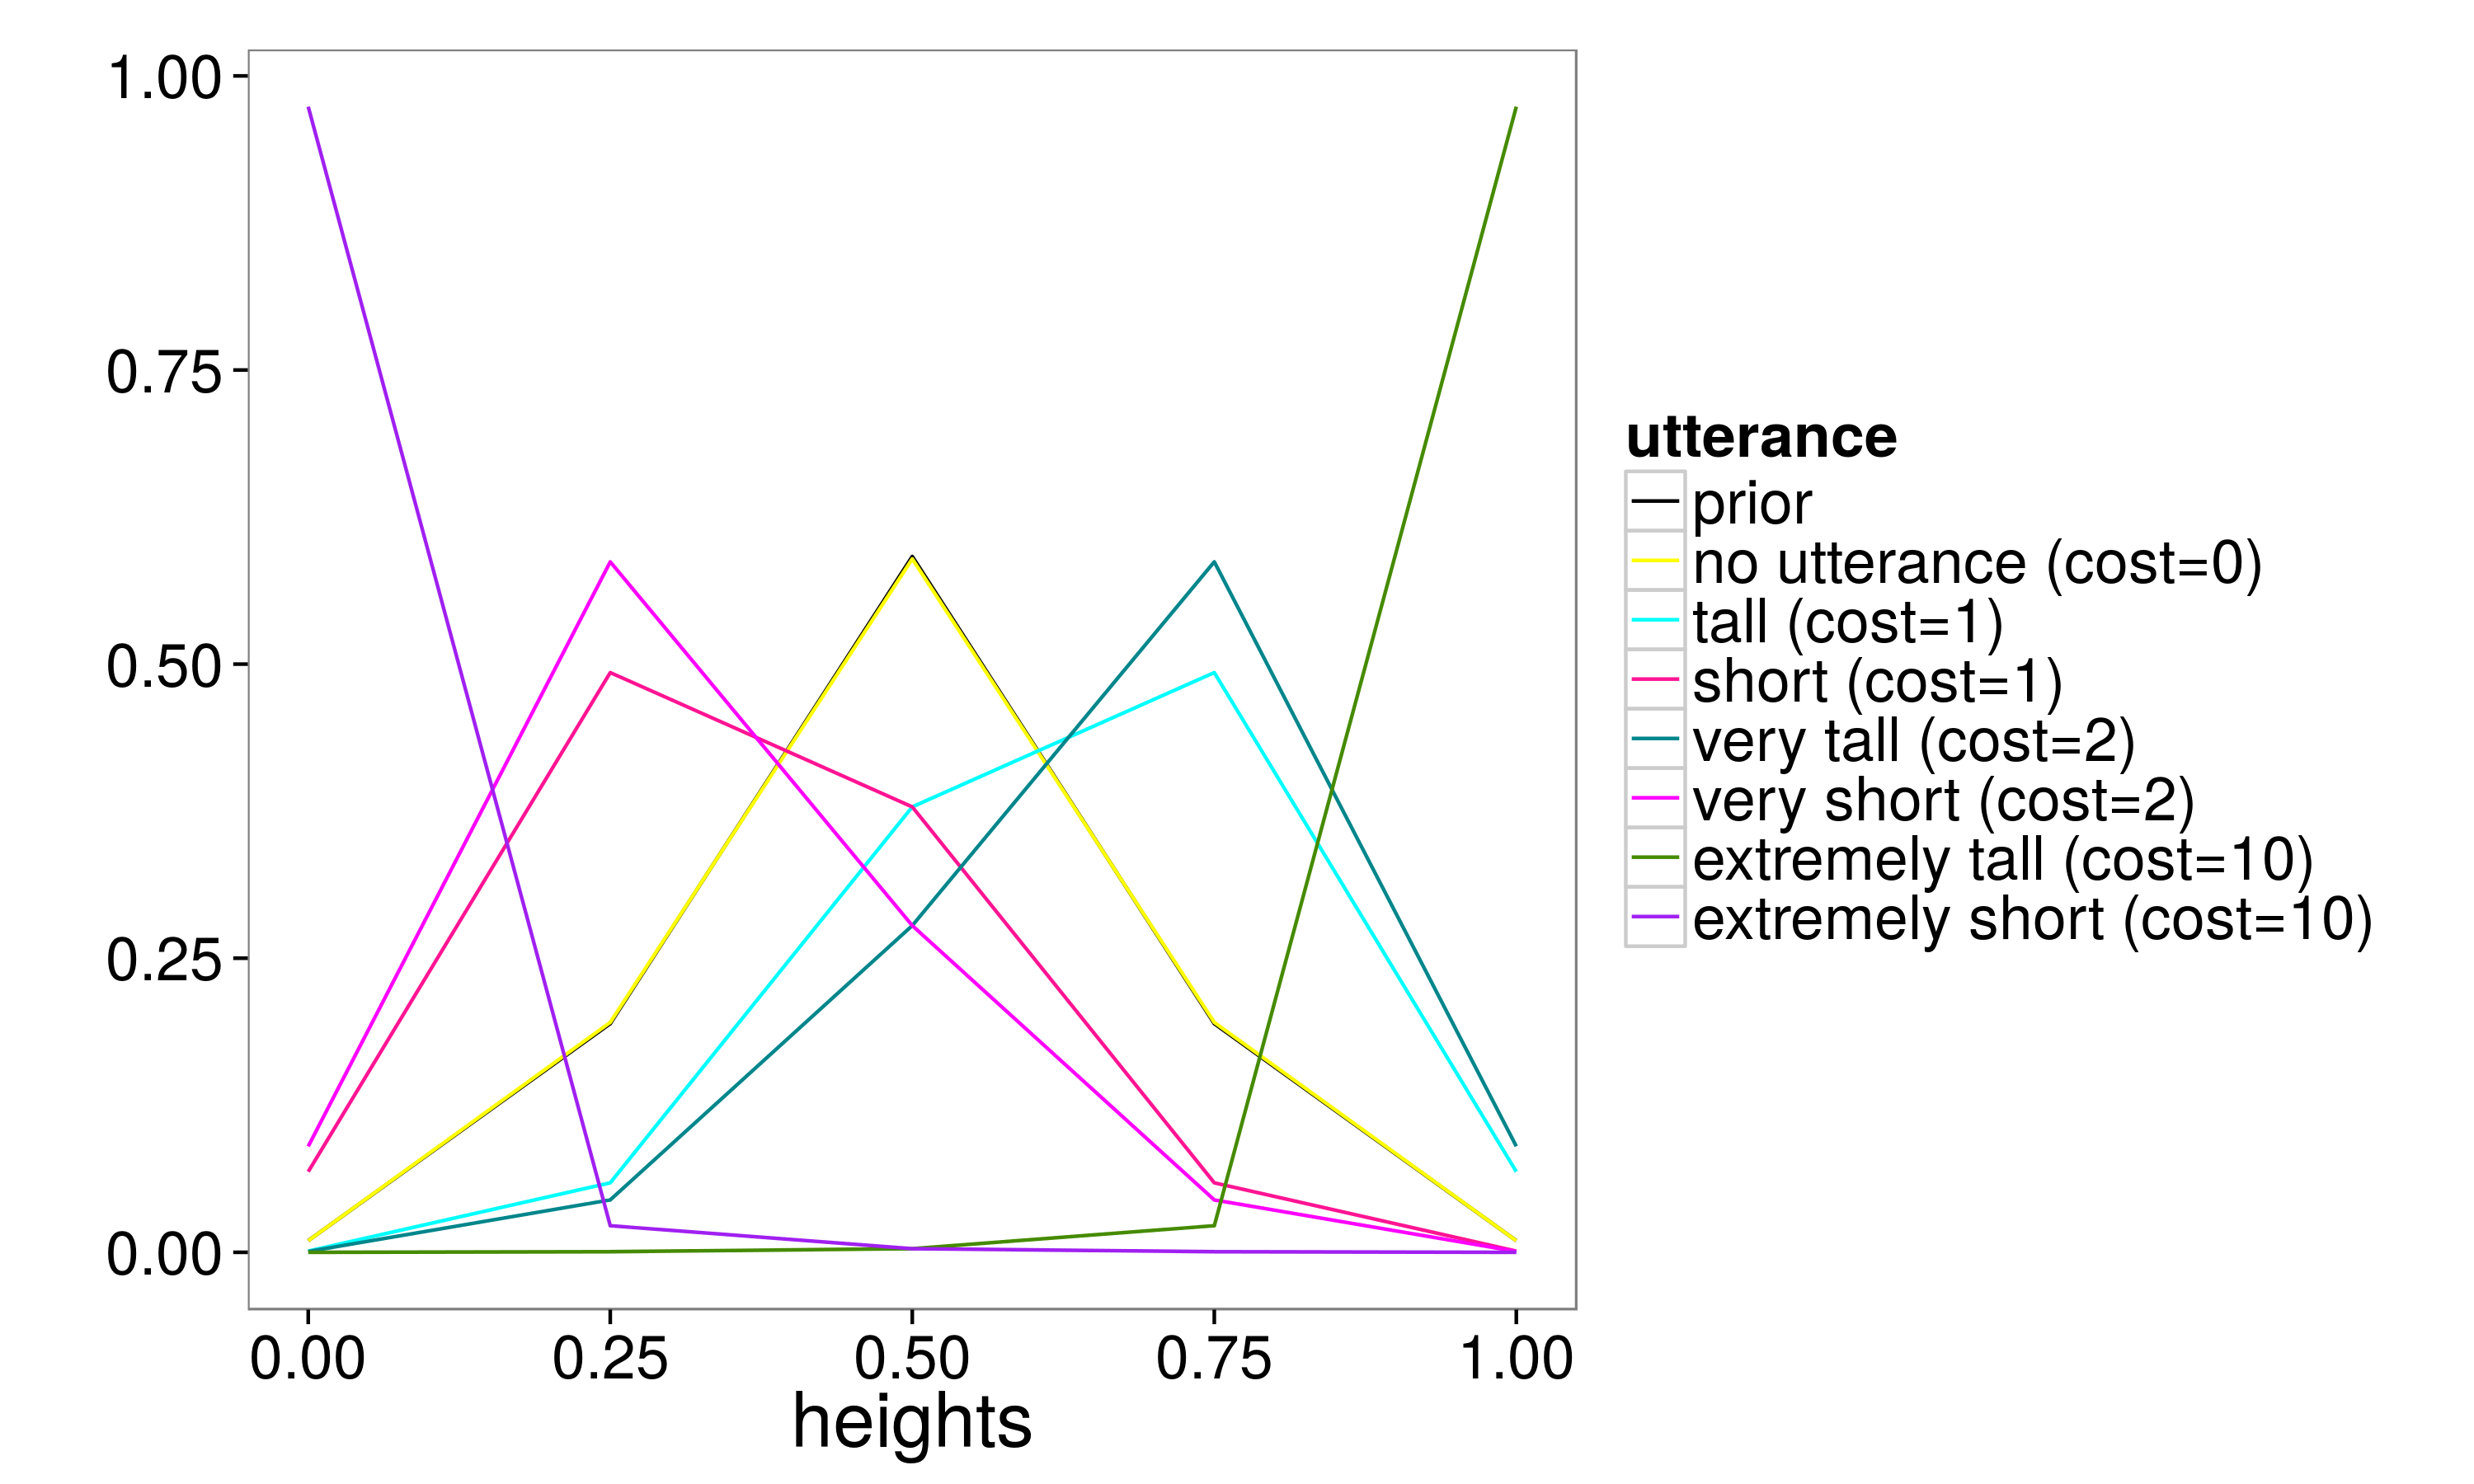
\includegraphics[width=0.48\textwidth]{analysis_files_for_writeup/images/model_results.png}
\end{center}
\caption{Modeling intensifiers as M-implicature: more costly intensifiers correspond to more extreme meanings. \todo{do this on a finer grid, so they look more like curves. also, do we need the negative polarity set (short)? would be clearer without them....} } 
\label{model}
\end{figure}


% - meaning as a function of cost?
%         - what is cost?
\subsection{Measures of cost}

%%% hard to follow!!! Maybe have this before Experiment 1.

Communicative cost, or markedness,
% markedness == communicative cost?
might be influenced by a variety of factors.

%However, f
For the purposes of this paper, we use quantities for costs that are straightforward to quantify: length (longer utterances are more costly)\footnote{We measure length in number of syllables, although length in characters (which might be a relevant source of utterance cost in a written format, as our partipants experienced) has similar
%(and in fact, slightly higher)
predictive power to syllable length in all of our analyses.}
%if we ran the same thing with audio, would syllables be a better predictor?
and frequency (rarer intensifiers might be less accessible and therefore harder to say or process).

%         - predictions
%                 - as cost increases, meaning becomes more extreme
We predict that as cost of an intensifier increases (i.e. as length increases and frequency decreases), its interpretation will become more extreme. This leaves open the question of their relative importance,
%discuss
how they combine,
%discuss
and what other factors %(such as discussed above)
might enter into cost.

%                 - (note: not clear on causal direction (yet))
% limitations of correlational studies in this domain
%%%%% make this clearer
\subsection{Limitations of these methods}
It should be noted that, since this is a correlational study, finding such a relationship would not confirm that an intensifier's cost \emph{actually causes} its meaning. This correlation is predicted by the model sketched above, but it might be predicted by a variety of other analyses of intensifiers and their meanings. Rarity in particular might be correlated with strength of meaning merely because more extreme meanings refer to less probable things in the world, are therefore talked about less, and therefore the words with those meanings will necessarily be rarer. Although it seems reasonable to suspect that word frequencies reflect the probabilities of the real-world concepts they describe, it might also be the case that improbable things are more likely to be commented on, and so to a certain extent the frequencies of words that describe rare concepts will be inflated. Even so, this confound exists only for word frequency and not for syllable length.
%citation?
The length of a word seems much less likely to reflect the real-word prevalence of the concept it refers to.

% ## Expt. 1
\section{Experiment 1}

The proposal detailed above predicts an association between measures of cost and strength of interpretations. In Experiment 1, we test this qualitative prediction %, and look at whether the cost associated with different intensifiers can predict their interpretations.
by eliciting free response prices from people and determining whether these prices are correlated with independent measures of utterance cost.

% - design and materials
\subsection{Method\footnote{The full experiment can be found at \url{http://web.stanford.edu/~erindb/degree-adverbs/experiments/exp5_2014-12-01/exp5.html}}}

40 participants with US IP addresses were recruited through Amazon's Mechanical Turk and paid \$0.4 for their participation.

We asked participants to provide judgements of prices based on a person's description of an object that included an intensifier (Figure~\ref{exp1-q}).
There were three categories of objects (\emph{laptop}, \emph{watch}, and \emph{coffee maker}) and 40 intensifiers (see Table~\ref{exp1-intensifiers}).
We chose intensifiers that have a wide range of frequencies and excluded intensifiers that are either more commonly used to signal affect than to signal degree (e.g. ``depressingly expensive'' might indicate a degree, but it mainly indicates affect) or are ambiguous between other parts of speech (e.g. ``super'' can be used as an intensifier, as in ``super expensive'', but it can also be used as an adjective, as in ``super hero'').
Each particpant gave price judgements for every intensifier-category pairing in randomized order, for a total of 120 price judgements.
We chose the domain of price and used only the adjective ``expensive'', because price constitutes a quantitative scale on which to measure the different intensifers.% and because we thought participants would have similar enough experience with the distributions over prices for these objects.
% come to think of it, we chose those exact objects because we thought they might have bimodal priors. possibly in future experiments where the analysis would be easier if people had the same distribution as one another, we should go to something that people purchase more frequently with less ambiguity about ``what kind''... like milk, or shampoo...?

\begin{figure}[ht]
\begin{center}
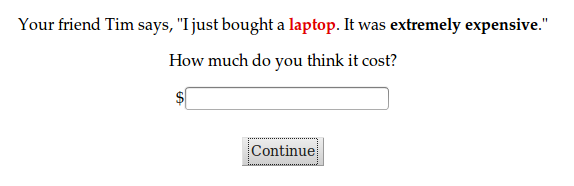
\includegraphics[width=0.4\textwidth]{analysis_files_for_writeup/images/exp1-q.png}
\end{center}
\caption{Screenshot from Experiment 1 target question.} 
\label{exp1-q}
\end{figure}

\begin{table}[ht]
 \begin{center}
 \footnotesize
  \caption{Intensifiers from Experiment 1, number of occurences in Google Web 1T 5grams corpus, and number of syllables.}
  \label{exp1-intensifiers}
  \begin{tabular}{ccc}
   \hline
   ngram & frequency & syllables \\
    \hline
    surpassingly & 11156 & 4 \\
    colossally & 11167 & 4 \\
    terrifically & 62292 & 4 \\
    frightfully & 65389 & 3 \\
    astoundingly & 73041 & 4 \\
    phenomenally & 120769 & 5 \\
    uncommonly & 135747 & 4 \\
    outrageously & 240010 & 4 \\
    fantastically & 250989 & 4 \\
    mightily & 252135 & 3 \\
    supremely & 296134 & 3 \\
    insanely & 359644 & 3 \\
    strikingly & 480417 & 3 \\
    acutely & 493931 & 3 \\
    awfully & 651519 & 3 \\
    decidedly & 817806 & 4 \\
    excessively & 877280 & 4 \\
    extraordinarily & 900456 & 6 \\
    exceedingly & 977435 & 4 \\
    intensely & 1084765 & 3 \\
    markedly & 1213704 & 3 \\
    amazingly & 1384225 & 4 \\
    radically & 1414254 & 3 \\
    unusually & 1583939 & 4 \\
    remarkably & 1902493 & 4 \\
    terribly & 1906059 & 3 \\
    exceptionally & 2054231 & 5 \\
    desperately & 2139968 & 3 \\
    utterly & 2507480 & 3 \\
    notably & 3141835 & 3 \\
    incredibly & 4416030 & 4 \\
    seriously & 12570333 & 4 \\
    truly & 19778608 & 2 \\
    significantly & 19939125 & 5 \\
    totally & 20950052 & 3 \\
    extremely & 21862963 & 3 \\
    particularly & 41066217 & 5 \\
    quite & 55269390 & 1 \\
    especially & 55397873 & 4 \\
    very & 292897993 & 2
  \end{tabular}
 \end{center}
\end{table}

\subsubsection{Corpus Methods}
%maybe have this a separate section? maybe not?

We used word length in syllables and word frequency as proxies for a word's cost (Table~\ref{exp1-intensifiers}).
The frequencies were collected from the Google Web 1T 5-grams database \cite{web1t5gram}\footnote{
We also ran the same analyses on frequency information collected from the Google Books American Ngrams Corpus \cite{books2011} as well, and found similar results.

In addition, we did the same using the bigram frequencies of ``\emph{[intensifer]} expensive'' rather than the unigram frequencies of the intensifiers alone. These data were much more sparse. For bigrams, we found no significant effects of surprisal using the books database and a negative effect using the web database. While the data for bigrams is more sparse, the fact that unigrams is a better fit might be an indication 
}
For all of the analyses that follow, we use \w{surprisal} or \w{self-information}, defined as the negative log probability of a word in the corpus, as the utterance cost measure. We do this so that our correlations for both utterance cost measures will be positive (if our findings are consistent with our hypothesis) and because \todo{reasons}. The syllable lenths of our intensifiers and the surprisals %\todo[inline]{say what surprisal is and why we care before using it.} 
were correlated, but not strongly so (r = 0.27).

% - results and discussion
\subsection{Results and Discussion}

%         - as cost increases, meaning becomes more extreme
If the meaning of an intensifier is stronger for higher cost intensifiers, we would expect to find that as frequency decreases and length in syllables increases, the prices participants give will also increase. We find that this is the case.
%% what's the alternative hypothesis?

\begin{figure}[ht]
\begin{center}
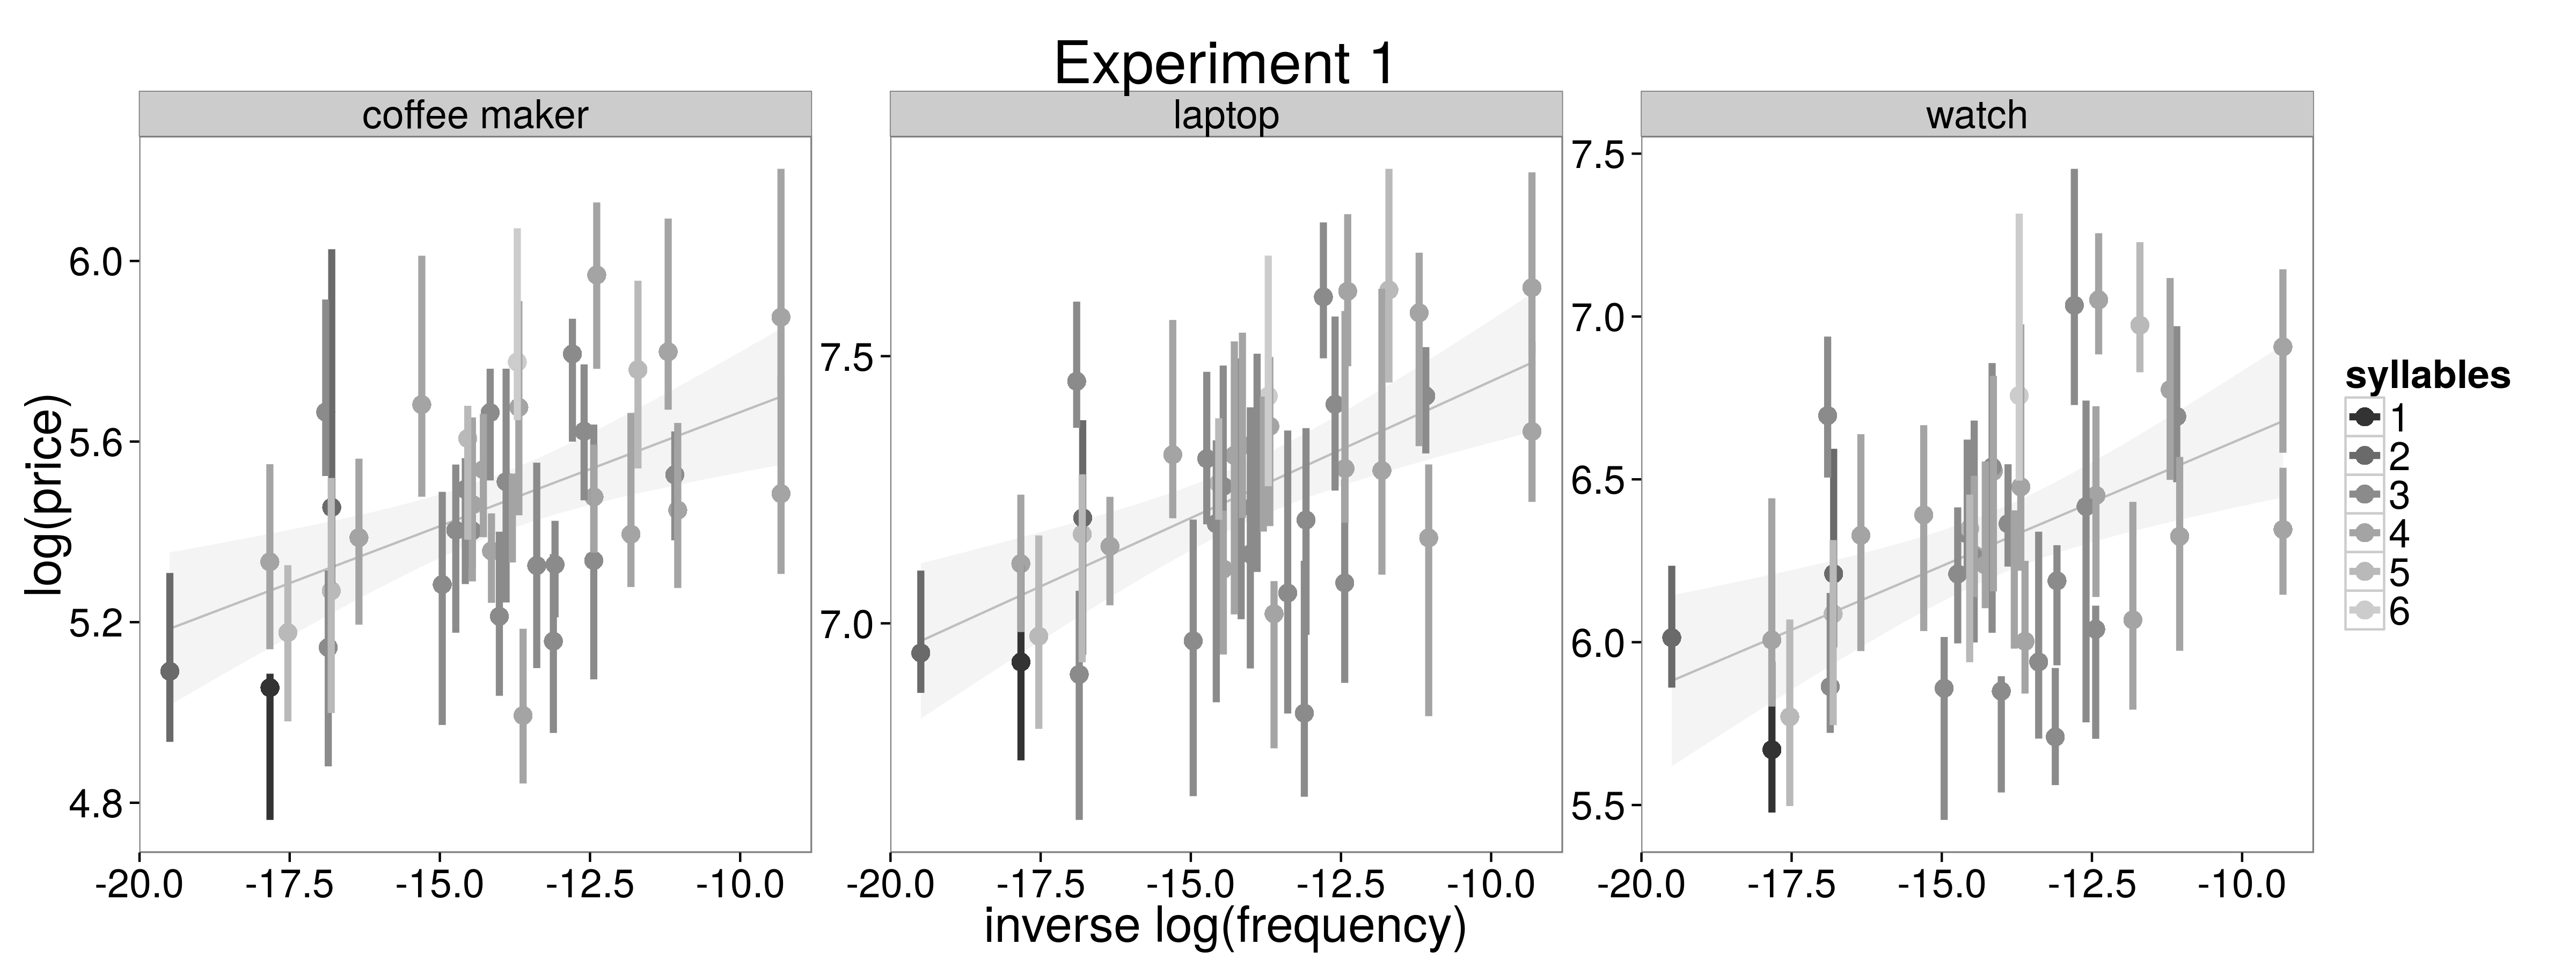
\includegraphics[width=0.48\textwidth]{analysis_files_for_writeup/images/exp1-plot.png}
\end{center}
\caption{Results of Experiment 1. As surprisal and length in syllables increase, participants' free response prices increased.} 
\label{exp1-plot}
\end{figure}

%%explain the main effects and the interaction: eg “we found significant main effects of surprisal and syllable length, such that more surprising and longer words were rated as more expensive”
%%integrate this last paragraph into the reporting of effects along the lines sketched above
We ran a linear mixed effects regression with centered fixed effects of syllables and surprisal and their interaction and random intercepts and slopes for syllables and surprisal for both participant and object.
%anything more complicated won't converge
We found significant main effects of surprisal ($\beta=0.0537, SE=0.00935, t=5.74, p<0.05$) and syllable length ($\beta=0.0931, SE=0.0182, t=5.112, p<0.005$), such that more surprising and longer words were rated as more expensive. We also found a significant interaction ($\beta=0.0193, SE=0.00515, t=3.75, p<0.0005$) between surprisal and syllable length.%, suggesting that \todo{...}.

So intensifiers that are more surprising and longer (and therefore are more costly to utter) also tend to be interpreted as having stronger meanings.

%         - support for m-implicature model
This is the consistent with the M-implicature model introduced in this paper.
%         - effect of design/dependent measure?
%% what does this mean?

%\todo[inline]{make a big deal}

\section{Experiment 2}

%replicated exp 1 using novel dependent measure and generalized to other (non quantitative) adjective scales

% ## Expt. 2
% - effect of design/dependent measure?
%         - motivate new design (e.g., more adjectives)
% - design and materials
% - results and discussion
%         - as cost increases, meaning becomes more extreme
%         - (more) support for m-implicature model
%         - causal direction?
%                 - cost -> meaning?
%                 - meaning -> cost?

\todo{why exp2?}

%why is exp. 2 necessary? motivate in one sentence. and how does this relate to the different dependent measure?

In Experiment 2, we extend our finding from Experiment 1 to other adjectival scales (in addition to ``expensive''). We use a ranking dependent measure which is more appropriate to non-quantitative scales and which we expect to be more sensitive to small differences in meaning.

\subsection{Method\footnote{The full experiment can be found at \url{http://web.stanford.edu/~erindb/degree-adverbs/experiments/exp4/exp4.html}}}

%% and were paid $.XX
30 participants with US IP addresses were recruited through Amazon's Mechanical Turk and paid \$0.40 for their participation.

%\todo[inline]{introduce the idea of the ranking measure first.}
Because arranging all 40 intensifiers on a computer screen would be difficult for participants, we divided the 40 intensifiers from Experiment 1 into four lists of 10 intensifiers each (Table~\ref{exp2-intensifiers}).
Each list was randomly paired with one of four adjectives (\w{old}, \w{expensive}, \w{beautiful}, and \w{tall}).
For each adjective-list pairing, participants were shown every combination of the 10 intensifiers and the one adjective.
They were asked to move the adjective phrases from the left to the right side of the screen, reordering the phrases from the lowest to the highest degree (Figure~\ref{exp2-q}).
Each participant completed four such trials, seeing all four lists and all four adjectives.
The pairings between list and adjective were randomized between participants.
The division of the intensifiers into lists of 10 was constant, i.e. the same 10 intensifiers were always shown together to simplify data analysis.

\begin{figure}[ht]
\begin{center}
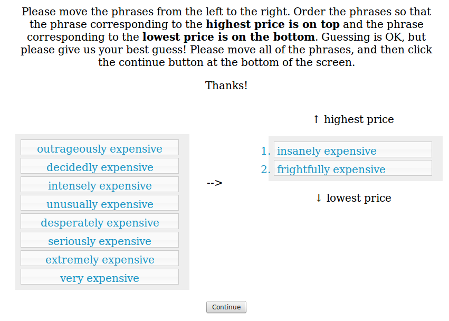
\includegraphics[width=0.4\textwidth]{analysis_files_for_writeup/images/exp2-q.png}
\end{center}
\caption{Screenshot from Experiment 2 target question.} 
\label{exp2-q}
\end{figure}

\begin{table}[ht]
\begin{center} 
\footnotesize
\caption{Intensifier Lists from Experiment 2: Rankings.} 
\label{exp2-intensifiers} 
\vskip 0.12in
%\scalebox{0.3}{
\begin{tabular}{cccc} 
\hline
List A    &  List B & List C & List D \\
\hline
surpassingly & colossally & terrifically & frightfully \\
astoundingly & phenomenally & uncommonly & outrageously \\
fantastically & mightily & supremely & insanely \\
strikingly & acutely & awfully & decidedly \\
excessively & extraordinarily & exceedingly & intensely \\
markedly & amazingly & radically & unusually \\
remarkably & terribly & exceptionally & desperately \\
utterly & notably & incredibly & seriously \\
truly & significantly & totally & extremely \\
particularly & quite & especially & very
\end{tabular}
%}
\end{center}
\end{table}

\subsection{Results and Discussion}

% fixed only:
% c.surprisal              0.31871746 0.02471029  12.8981699  4.609137e-38
% c.syllables              0.43704201 0.06580015   6.6419605  3.095379e-11
% c.surprisal:c.syllables  0.04097697 0.02360147   1.7362040  8.252777e-02

We ran an ordinal
%mixed effects
regression with centered surprisal and syllable lengths and their interaction as fixed effects.
\todo{random effects?}
We again found main effects of surprisal ($\beta=0.319, SE=0.0247, t=12.9, p<5e-38$) and syllable length ($\beta=0.437, SE=0.0658, t=6.64, p<5e-11$), but only a trending interaction ($p=0.0825$).
%and random intercepts of intensifier list\footnote{The random intercept for intensifier list helps to standardize the rankings across the different intensifier lists. If the spacing between predictors were roughly the same across the different lists, then adding a constant value to the rankings for every element in a particular list would allow us to compare that list to another.} and adjective and random by-participant and by-list slopes to predict the ranking that participants gave the adjective phrase (the highest ranked adjective phrase in a trial got a ranking of 10, the lowest ranked adjective phrase got a ranking of 1). We found main effects of surprisal (estimate=0.46, p=4.8e-8) and syllable length (estimate=0.68, p=3.6e-10) and a significant interaction (estimate=0.079, p=0.025). Regressions on subsets of the data for each intensifier list were mostly similar, except that for intensifier lists C and D, which had smaller syllable ranges, the effects of syllable length and its interaction with surprisal were sometimes insignificant or in the opposite direction. Results were very similar across the four different adjectives.

\begin{figure}[ht]
\begin{center}

\includegraphics[width=0.48\textwidth]{analysis_files_for_writeup/images/exp2-plot.png}
\end{center}
\caption{Results of Experiment 2. As surprisal and length in syllables increase, participants' rankings increased.} 
\label{exp2-plot}
\end{figure}

Overall, we again found that participants assign stronger interpretations to intensifiers with higher surprisals and higher syllable lengths.

\section{General Discussion}

Motivated by an extention of \citeA{lassiter}'s scalar adjectives model which allows for a single semantics for all intensifiers with variation determined by M-implicature, we found an association between the length and surprisal of an intensifier and the strength of degree that it indicates.

We provide evidence that intensifier meanings are not mapped arbitrarily to word forms, but depend systematically on the length and frequency of distribution of those word forms.

%%%maybe move that to the discussion
%make it sound like ``this is a reasonable thing to do.
%then in the discussion say, ''that was reasonable, but there are other reasonable things. for example:
%%%% 
%justine: ``C(u) is the psychological cost of an utterance, potentially determined by factors such as the utterance's frequency, availability, and complexity.
%
%%%maybe this should be a footnote:
%%%%%%The extent to which a degree adverb (e.g. \w{terribly}) takes a degree interpretation (e.g. ''a lot`` as opposed to ''this sucks``) can be approximated by the extent to which it 
%the number of different types of adjetives that it coocurs with
%freely collocates with a variety of adjectives, since adverbs that are more qualitative will have more restricted collocations.

The relationship between surprisal and interpretation might be causal, and the causal direction might be that the rarity of the word causes it to be costly to use and therefore to correspond to a stronger meaning, as in our hypothesis.
However, the causal direction could also be the opposite.
Perhaps the fact that an intensifier has a stronger meaning (which it may have gotten completely arbitrarily) causes it to be used only in extreme and unusual circumstances.

Further work will provide more thorough tests of our model hypothesis, for example determining whether length and frequency are causes of intensifier meanings, and investigate to what extent the M-implicature described in our hypothesis is consistently computed online and to what extent it might be conventionalized.

We could also investigate other sources of commicative cost. \cite{peters} %Peters (1994)
notes that, since intensifiers often originate as qualitative adverbs and gradually shift to being primarily adverbs of degree (e.g. terribly once only carried the qualitative meaning of ``bad and frightening'', but now almost exclusively means simply ``a lot''), interlocuters might have to resolve ambiguity about which sense of the adverb is intended and that resolving this ambiguity could be cognitively demanding. So intensifiers that are newer and less conventially used to signal degree, like \w{skyscrapingly}, would incur higher communicative cost to the comprehender (in disambiguating) and to the speaker (in choosing a less common meaning, or creatively generating a new intensifier) than something more commonly used to signal degree, like \w{very}.\footnote{The extent to which an adverb is used as an intensifier as opposed to as a qualitative adverb can be approximated by the number of types of adjectives an adverb can coocur with. The more freely it is able to pair with arbitrary adverbs, the more likely its conventional meaning is one of degree as opposed to quality.}

% ## General Discussion
% - m-implicature theory of intensifier interpretation
%         - benefits
%                 - single intensifier semantics
%                 - works with lassiter & goodman adjectives story
%         - model in brief?
% - further applications
%% further questions!

%We first introduce a model of intensifiers which predicts an M-implicature \cite{levinson}, where more costly adjective phrases will be associated with more extreme meanings. We then confirm in two experiments that interpretations of English intensifiers in adjective phrases are indeed higher for more costly intensifiers. We conclude with a discussion of other possible explanations for this correlation and future directions.

%%%spell out further and bring back to big questions from the intro :)

% it's probably too early to 
% this is a different kind of association than people have talked about.

%in general discussion / conclusion should address again the thing from the intro, also talk about other aspects of meaning (eg affect), issues with our results, and some future directions.

In conclusion, we found that frequency and syllable length can predict the interpretations of adverbs, %and manipulating frequency in turn changes the interpretation,
providing evidence that effective meaning is a combination of both arbitrary convention and non-arbitrary factors mediated by pragmatic inference.

%\todo[inline]{revisit our point and summarize briefly our results.}

%\todo[inline]{discuss other probable contributions to intensifier meaning: polarity, affect, others?}

%\todo[inline]{if room could say something about next steps. also relation to other's work on meaning.}

%\todo[inline]{close by restating our big picture point, that effective meaning is a combination of both arbitrary convention and non-arbitrary factors mediated by pragmatic inference.}

%\todo[inline]{conclusion}

\section{Acknowledgments}

\bibliographystyle{apacite}

\todo{fill in missing information for references}

\setlength{\bibleftmargin}{.125in}
\setlength{\bibindent}{-\bibleftmargin}

\bibliography{intensifiers}

\end{document}
